\documentclass[a4paper,11pt,onecolumn]{article}
\usepackage[hscale=0.8,vscale=0.9]{geometry}
\usepackage[parfill]{parskip}
\usepackage{amsmath}
\usepackage{amsfonts}
\usepackage{graphicx}
\usepackage{subfigure}
\usepackage{wrapfig}
\usepackage{amssymb}

\newcommand{\eat}[1]{}

\begin{document}
\include{weld-defns}
\title{Research Statement}
\author{Niranjan Balasubramanian}
\maketitle

My research spans two broad areas: Information retrieval and Natural Language Processing. Applications like Question answering, event extraction and summarization systems, and web search providing easy access and organization to the vast amounts information on the web. These challenging applications require computer systems to extract, understand and reason with knowledge present in natural language texts. This long-standing Artificial Intelligence (AI) vision has tremendous societal and scientific impacts. My research is motivated by this vision and aims at building large scale open domain knowledge targeted towards specific applications.

Consider a system answering a 4th grade science question:  ``Which is the best conductor of electricity? (A) metal fork (B) rubber boat''. The system needs access to the knowledge that i) a metal fork is made of metal, ii) metals conduct electricity, and iii) properties of a metal apply to things made of metal and reason with this knowledge to arrive at the answer. Consider an event extraction system that is "reading" an article about an arrest event. If the system had knowledge about what a typical arrest event is -- i.e., who the key actors are and what their roles are -- then it can use that information to identify the salient pieces to extract from the article. 

My current research focuses on developing methods for extracting such large scale open-domain knowledge and robust mechanisms for applying this knowledge. For wide applicability, I target methods that meet the following design goals: Scale to arbitrary domains, model semantics without ambiguity, and generalize to unseen contexts. I use Open Information Extraction (Open IE) techniques to extract open-domain relations and representations augmented with semantic classes to reduce ambiguity and improve generalization.

My research methods are centered on identifying the core aspects of the problem space through careful analysis of existing systems and data. For instance, in my work on event schemas, I analyzed output from previous system and identified the key shortcomings of underspecified representations. The insights led to a better representation that vastly improved the quality of the schemas. In my work on mobile search, I conducted a systematic study of data transfer costs in cellular networks. This study identified a key energy inefficiency, which spawned a large body of research aimed at minimizing its impact.~\footnote{This work has more than 350 citations.} 

Here I describe some of my research and lay out my vision for future work.

{\bf NLP [EMNLP 2013, AKBC-WEKEX 2012, 2013]}

{\bf Modeling Events}

Event schemas that specify actors and their roles within events are widely used in event extraction. Figure~\ref{fig:arrest} shows an example arrest schema. The key actors are an arresting agent who arrests and charges a suspect, a lawyer who represents the suspect and a judge who rules on the case. My research aims to automatically generate these schemas from text with no manual effort with a specific focus on generating coherent schemas.

The main premise behind my work is that an accurate model of co-occurring actors and their actions can provide a basis for automatically generating schemas. The main challenge is in defining a suitable representation for the actions. My analysis of the output from a previous system showed that simpler (subject, verb) and (verb, object) pairs are underspecified representations that split critical context. In response, I developed an Open IE triple-based solution that uses a (Arg1, Relation, Arg2) triple that captures more specific information about the actions and reduces ambiguity. However, this reduction in ambiguity comes at a cost of increased sparsity and reduced generalization. 
\begin{wrapfigure}{r}{0.4\textwidth}
	\vspace{-2ex}
	\begin{center}
	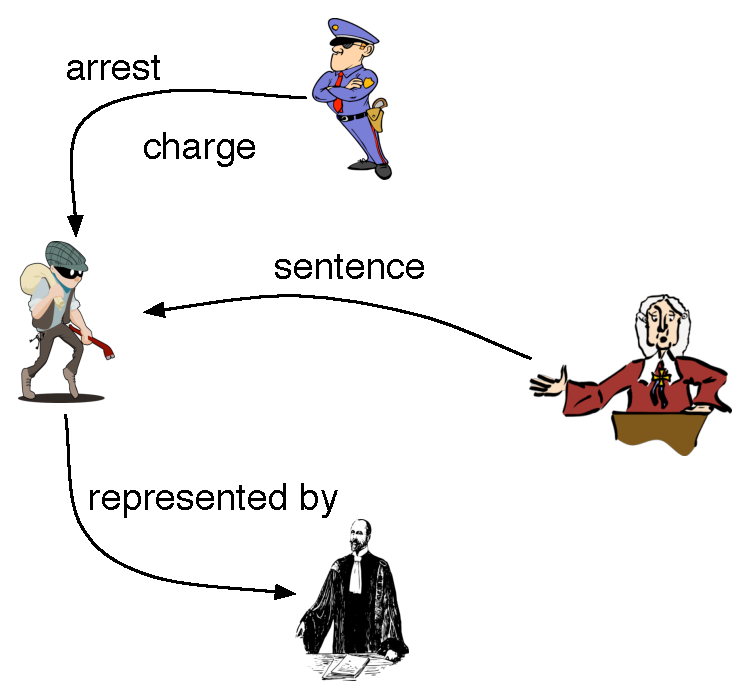
\includegraphics[width=2.5in,height=2in]{figures/arrest-scenario} 	
	\vspace{-2ex}
	\caption{\label{fig:arrest} {\small Arrest schema: A model for an arrest scenario including key actors, the police, the suspect, judge etc. and their roles.}}
	\vspace{-2ex}
	\end{center}
\end{wrapfigure}
To counter this issue, I represent arguments using semantic classes, which allows the model to generalize beyond the specific entities to new unseen contexts. The relational co-occurrence model (Rel-grams) built over this triple representation yields a form of entailment type knowledge~\cite{balasubramanian-akbc12} and produces schemas that are more coherent than state-of-the-art systems~\cite{balasubramanian-emnlp13}.

{\bf Question Answering}

Achieving human-level performance on tasks that require intelligence has a long tradition in the history of AI. As one of the foundational members of the Allen Institute for Artificial Intelligence, I am co-leading efforts to design and develop a QA system that is capable of passing a 4th grade science exam.~\footnote{I also contribute to the long term research planning efforts and earlier co-wrote grant proposals with Dr. Oren Etzioni to obtain funding on earlier versions of this project.} This is an exciting long-term research project that seeks to address several fundamental challenges in representation, extraction and reasoning all in the context of a single task. 
\begin{wrapfigure}{l}{0.6\textwidth}
	\begin{center}
	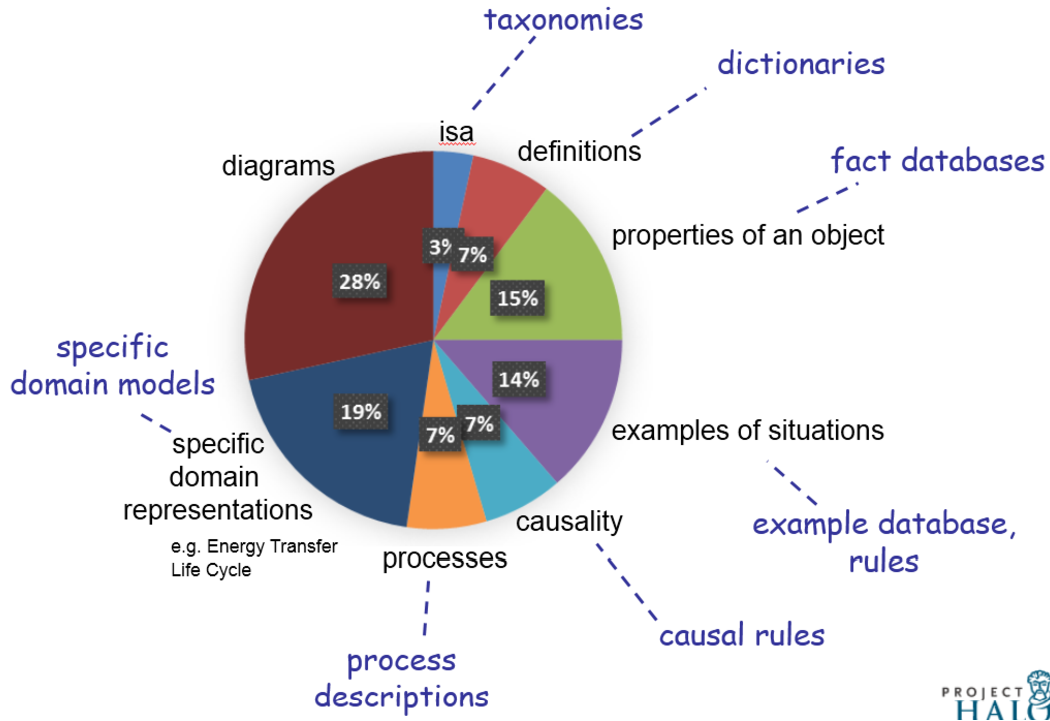
\includegraphics[width=3in,height=2in]{figures/akbc} 	
	\vspace{-2ex}
	\caption{\label{fig:akbc} {\small Knowledge Requirements for passing a 4th Grade Science Exam}}
	\vspace{-2ex}
	\end{center}
\end{wrapfigure}

As a first step in this task, we studied the knowledge requirements for passing a 4th grade science exam~\cite{clark-akbc13}. The knowledge requirements summarized in Figure~\ref{fig:akbc} shows that this is a challenging task requiring a wide range of knowledge and robust reasoning methods. In addition to factual knowledge (e.g., iron conducts electricity), we identify three other types of useful knowledge: 1) Definitional knowledge, 2) Domain knowledge expressed via general purpose relations such as cause/effect, entity/function, 3) Implications representing domain and background knowledge (e.g., animal breathes oxygen $-$enables$\rightarrow$ animal make energy), and 4) Qualitative domain models (e.g., Reasoning with predator-prey models: If population of snakes rise, what happens to the population of frogs?).

We are building a wide array of solutions to address these difficult challenges. We extract definitional and general purpose relations such as cause/effect and entity/function using hand-generated lexico-syntactic patterns that exploit strong regularities in language. We use Open IE style relations to represent information but expand them to cover nested relations. In addition, we also use facts extracted using a state-of-the-art Open IE extractor. Our preliminary experiments show about 15\% improvement over simpler BOW baselines.

{\bf Information Retrieval [SIGIR 2010, CIKM 2009, IMC 2009, CoNext 2012]}


{\bf Combining Alternatives}

The IR research community continuously develops query representations, retrieval models, and various ranking algorithms. As part of my thesis, I developed a dynamic query-dependent approach for combining different alternatives. The main premise behind my thesis is that different alternatives work well for different queries. For example, a navigation query (intent to visit a specific url) is well served by user click based features, whereas a informational query is better served by query-document match features. If we can select the best choice(s) for a given query, then we can further improve retrieval performance. 

To this end, I developed a novel method that estimates the relative performance of the alternatives with respect to a baseline using easy to compute retrieval features~\cite{balasubramanian-sigir10a}. The key insight behind this method was that accurate estimation of the absolute effectiveness value was not essential. The estimation only needed to induce a good ordering of the available alternatives. This relative estimation method outperformed using the single best alternative for query representations~\cite{balasubramanian-sigir10b} and standard fusion methods for combining ranking functions~\cite{balasubramanian-sigir10c}. 


{\bf Topic Pages}

As an alternative to the typical web search paradigm, I built a system that automatically generates wikipedia like pages for queries~\cite{balasubramanian-icsc2010}. The primary challenge here is to identify the salient aspects pertaining to the query topic. I used web search logs to build diverse aspect models on topics. To generalize to topics beyond those that are observed in the search logs, I generalized the aspect models to include information from related topics. A second challenge here is to extract and organize information pertaining to the diverse aspects in a coherent fashion. I built a sentence extractor that identifies most typical connection between the topic and its aspect and used simple word-precedence models to organize the retrieved sentences. The resulting topic pages outperformed state-of-the-art summarization systems in terms of grammaticality, salience and coherence.

{\bf Mobile Search}

I studied the impact of system constraints on web search from mobile phones. I conducted a systematic study of how network activity consumed energy in mobile phones. My study revealed that energy consumption also depended on inter-transfer times in addition to the size of the data being transferred~\cite{balasubramanian-imc09}. Based on this insight, I designed interaction strategies that reduced the energy consumption of web search applications. In addition to improving the energy efficiency of web search, the key finding in this work led to a large body of work aimed at addressing the energy inefficiency.

I also worked on {\em FindAll}, a mobile search engine aimed at improving local availability of previously visited documents. Because indexing on the phone is expensive, the system must balance local availability against resource usage and energy consumption. Using actual search logs from mobile users, we learned user-specific re-finding patterns to predict when a user is likely to re-find documents. Using this predictive model, FindAll selectively indexes documents when cost of indexing is lower than cost of re-finding the document over the network. Evaluations show that FindAll dramatically improves local availability for heavy users without increasing the energy costs.

{\bf Future Work}

I am interested in three veins of research for future work. First, I am interested in continuing my work on extracting open-domain knowledge from text. In particular, I want to extract rich descriptions of open-domain events that can serve as back-ground knowledge during extraction. Second, I am interested in developing methods that can reason with automatically extracted knowledge. Third, I am interested in applying semantic resources to improve information retrieval techniques.

{\bf Event Extraction using script-like knowledge}

The goal of event extraction is to identify events mentioned in texts and extract key actors and their actions. Building an automatic system for this task is challenging in many respects. In addition to a model of the key actors and their actions, the system should also fill in missing connections and resolve ambiguous references. Consider the sentences ``John went to Bill's restaurant. [He] ordered a steak. [He] paid \$50 in cash for [the meal]''. When we read these sentences, we easily identify that the key actors are John, the restaurant, a waiter who took the order etc. Note that the waiter was never mentioned in the text. Also, we are able to infer that the pronouns in the sentences all refer to John, [the meal] refers to the steak, and going a step further we can even infer that John probably ate the steak before paying for the meal. To do this automatically, we need a rich model of background knowledge about people eating in restaurants. 

Scripts were proposed as a general purpose description of events or scenarios. They include the key actors, their actions, and causal and temporal relationship between the different actions~\cite{schank-scripts75}. My prior work on open event schemas provide a starting point for building scripts but many challenges remain: First, we need extractors for the actors and their actions -- i.e., patterns that can be used to extract from new texts. The key challenge here is to expand the schemas by identifying the different ways in which certain actions and actors are specified in texts. I intend to leverage existing semantic resources such as Freebase, YAGO and NELL to expand the descriptions of actors and actions. Second, the system needs to handle entity and event co-reference. This presents an opportunity for joint modeling of entity and event co-reference. Third, schemas do not include causal and temporal ordering of the actions in a scenario. This is challenging because causal and temporal links can be implicit. However, the explicit links can be identified more reliably especially when combined with structural constraints such as transitivity and can be aggregated to identify implicit links.

A common theme underlying all these challenges is extrapolating and generalizing from knowledge that can be identified with high precision either from text or from other sources.  Addressing these challenges requires development of high precision methods as well as representations that allow for generalization of the knowledge to new unseen contexts. 


{\bf Reasoning with Automatically Extracted Knowledge}

Reasoning with knowledge extracted from texts require robust mechanisms to handle the inherent uncertainty, redundancy, and vocabulary mismatch issues. I am interested in approaches that preserve a deductive style of reasoning as much as possible but revert to feature-based textual entailment style reasoning when necessary. I believe this combines the best of both worlds -- explaining the reasoning, showing where the current knowledge is lacking or where textual reasoning is required, while also retaining the robustness of the entailment style methods. 
%The question answering task is a great testbed to test these ideas. %In addition to providing an explanation of the reasoning, this approach explicitly highlights the shortcomings of the extracted knowledge.

To this end, I am interested in building a probabilistic reasoning framework. Specifically, I want to model question answering as a marginal inference problem in a Markov Logic Network (MLN) with text-based implications as first-order rules and Open IE style relations as evidence. Different from traditional applications of MLNs, the knowledge and rules here are textual, which result in gaps from vocabulary mismatch. To address these gaps, I will build a search solution that uses coarse but fast methods to locate plausible gaps and bridge them using deeper (more expensive) textual entailment techniques. The key challenges here include keeping the search space tractable and to have broad coverage entailment methods to handle lexical variations. 

%Reasoning with knowledge extractedd from texts requires robust approaches. However, past attempts at producing robust approaches has mainly resulted in everything in the kitchen sink style approaches. This has led to measured progress in textual entailment tasks, but they haven't shed much insights into the properties of the systems themselves or on the problem space. In contrast, I am interested in approaches that preserve the deductive style of inference as much as possible while falling back to distributional methods to bridge gaps but within the inference framework. This I believe combines the best of both worlds -- retains the robustness of the entailment style methods while also explicitly showing where the current knowledge is lacking or where textual reasoning is required. The question answering project is a great testbed to test these ideas.

{\bf Information Retrieval}

I am also interested in exploiting semantic knowledge for Information retrieval. In the past, IR applications have had mixed success with using semantic resources. The key limiting factor was the coverage of the resources used and scalability of the methods. Recent advances in large scale language processing and knowledge extraction techniques provide an ideal opportunity to test integration of semantics. Open Information Extraction presents an ideal starting point. It provides fast and a shallow representation of salient information in a corpus that can be used to improve retrieval. 


\eat{
%Resolving co-reference is a challenging problem that requires broad semantic knowledge~\cite{}. Consider the following sentence: ``[People] travel to see their [families] when [they] find cheap flights to take [them]". [they] can resolve to families or [people]. Resolving pronouns in this sentence requires the system to know that the entity that travels is the one that is likely to find flights. Rel-grams provides a framework for aggregating this kind of background knowledge. One of the key challenges is the precision/recall trade-off. Past attempts at improving co-reference by adding semantics have mixed results because they either lack coverage or are too imprecise due to over-generalization. Rel-grams addresses this to some extent by including more context to improve accuracy and semantic classes to improve generalization. [But more needs to be done... What?]

Question answering for passing grade science exams requires extraction and reasoning with implications knowledge. The work on Rel-grams provides a starting point but is seriously limited especially in terms of the amount of context captured. For example, consider the question about 
...\\
...\\
...\\


Reasoning with semantic resources constructed from texts requires robust approaches. However, past attempts at producing robust approaches has mainly resulted in everything in the kitchen sink style approaches. This has led to measured progress in textual entailment tasks, but they haven't shed much insights into the properties of the systems themselves or on the problem space. In contrast, I am interested in approaches that preserve the deductive style of inference as much as possible while falling back to distributional methods to bridge gaps but within the inference framework. This I believe combines the best of both worlds -- retains the robustness of the entailment style methods while also explicitly showing where the current knowledge is lacking or where textual reasoning is required. The question answering project is a great testbed to test these ideas...\\

Lastly, I am interested in exploiting semantic resources for Information retrieval. In the past, IR applications have had mixed success with using semantic resources. The key limiting factor was the coverage of the resources used...\\
}
{\small
\bibliographystyle{plain}
\bibliography{../research-statement,../kia}
}
\end{document}


\eat{As a first step in this challenging task, we studied the knowledge requirements for passing this exam~\cite{clark-akbc13}. The analysis presented several critical insights into the challenges that lay ahead. Figure~\ref{fig:knowledge-wheel} shows the required knowledge categories as a wheel. In addition to factual knowledge (e.g., iron conducts electricity), we identify three other types of useful knowledge: 1) Definitional knowledge: Terminology questions often test the ability of students to match terminology to its description. 2) Domain knowledge: A wide variety of domain knowledge expressed via general purpose relations such as cause/effect, action/purpose, entity/function and object/property. 3) Implications: To answer many questions the system requires knowledge represented as implications (e.g, animal breathes oxygen $-$enables$\rightarrow$ animal make energy). 4) Domain models: Modeling questions involve ability to reason with certain types of models (e.g. Reasoning with predator-prey models: If population of snakes rise, what happens to the population of frogs?). }
